\section{Experiments} \label{sec:eval}
\subsection{Experimental Setting}
\fakeparagraph{Dataset}
\gaia{}\cite{mialon2023gaia} is a benchmark designed to evaluate general-purpose AI assistants through 300 test and 165 validation real-world, scenario-based questions covering daily tasks, tool usage, reasoning, multimodal inputs, and web browsing. While these tasks may appear straightforward for humans, they remain highly challenging for advanced AI systems. Each question is associated with a unique ground-truth answer, and model performance is measured using exact match accuracy.

\fakeparagraph{Metrics} 
We adopt the evaluation protocol of the \gaia{} benchmark, which relies on exact match accuracy. The main metric is \textit{Pass@N}, defined as the probability that at least one correct solution appears among $N$ independent execution. This metric, commonly used in tasks like code generation, captures whether the model can generate a valid solution at least once. Unless otherwise specified, our experiments report the average \textit{Pass@1} score, indicating the model’s ability to produce a correct answer in a single task run.

\fakeparagraph{Baselines}
For a comprehensive evaluation, we compare our system against various baselines from three primary types: agentic models (Search-o1-32B, WebThinker-32B, WebDancer-32B, WebShaper-32B); closed-source frameworks (Langfun~\cite{Peng_Langfun_2023}, TraseAgent~\cite{trase2024trase}, Deep Research~\cite{deepresearch}, h2oGPTe~\cite{h2oGPTe2024h2oGPTe}, and Desearch~\cite{desearch}); and open-source systems (OWL~\cite{owl2025}, TapeAgent~\cite{bahdanau2024tapeagentsholisticframeworkagent}, AutoAgent~\cite{tang2025autoagent}, Open Deep Research~\cite{opendeepresearch}, Smolagents~\cite{smolagents}, OAgent~\cite{oagent}, and MiroFlow~\cite{miroflow}). This selection captures a broad range of the latest developments in both proprietary and open multi-agent systems, establishing a robust benchmark for assessing the performance.

\subsection{Main Results}
The results presented in Table 1 offer several key insights into the performance of various agent frameworks on the \gaia{} benchmark. Our proposed method achieved an average score of 75.2 at Pass@1 and 82.4 at Pass@3, demonstrating competitive results against all other evaluated frameworks, including both closed-source and open-source alternatives. This outcome underscores the robustness and effectiveness of our agent's design.

For Level 1 tasks, our method achieved a score of 86.8, matching the top-tier performance and demonstrating the reliability of our low-level agents and their underlying system utilities. Compared to leading closed-source solutions such as Langfun (71.5) and MiroFlow (74.5), our approach shows substantial improvements in overall average performance and maintains superior accuracy across both Level 1 and Level 2 tasks. Notably, the highest-performing solutions predominantly leverage Claude-family models, underscoring the importance of foundation model selection. These results collectively validate the effectiveness of our framework for general-purpose agent applications.

We publicly run our agent against GAIA testset, and obtain a relatively high score of 67.1. Please refer to GAIA's official leaderboard\footnote{\url{https://huggingface.co/spaces/gaia-benchmark/leaderboard}}. Regarding Open Deep Research ~\cite{opendeepresearch} and Smolagents \cite{smolagents}, their reported results were directly adopted from OAgents \cite{oagent} due to the substantial computational resources required for replication.

\begin{table}[!thb]
\centering
\caption{Performance of various agent projects on the GAIA benchmark.}
\label{tab:related}
\begin{tabular}{lcccccl} 
\toprule
\midrule
\textbf{Framework} & \textbf{Pass@1} & \textbf{Pass@3} & \textbf{Level 1} & \textbf{Level 2} & \textbf{Level 3} & \textbf{Model Family} \\
\midrule
\multicolumn{7}{l}{\cellcolor[RGB]{235, 228, 230}{\emph{Agentic Model}}} \\
\midrule
Search-o1-32B
& 39.8 & & 53.8 & 34.6 & 16.7 & QwQ-32B \\
WebThinker-32B
& 48.5 & & 56.4 & 50.0 & 16.7 & QwQ-32B \\
WebDancer-32B
& 51.5 & 64.1 & 61.5 & 50.0 & 25.0 & QwQ-32B \\
WebShaper-32B
& 53.3 & 61.2 & 69.2 & 50.0 & 16.6 & QwQ-32B \\
\midrule
\multicolumn{7}{l}{\cellcolor[RGB]{235, 216, 221}{\emph{Closed-source Agent Frameworks}}} \\
\midrule
Langfun
& 71.52 & & 83.02 & 68.60 & 57.69 & Claude-3-7 etc.\@ \\
TraseAgent
& 70.30 & & 83.02 & 69.77 & 46.15 & Claude etc.\@ \\
DeepResearch
& 67.36 & & 74.29 & 69.06 & 47.60 & - \\
h2oGPTe
& 63.64 & & 67.92 & 67.44 & 42.31 & Claude-3.5  \\
Desearch
& 56.97 & & 71.70 & 58.14 & 23.08 & GPT-4o \\
\midrule
\multicolumn{7}{l}{\cellcolor[RGB]{235, 181, 195}{\emph{Open‐source Agent Frameworks}} }\\
\midrule
OWL
& 69.1 &  & 84.9  & 67.4 & 42.3 & Claude-3-7 etc.\@ \\
TapeAgents
& 55.8 & & 71.7 & 53.5 & 30.8 & Claude-3-7 etc.\@ \\
AutoAgent
& 55.2 & & 71.7 & 53.4 & 26.9 & Claude-3-5 etc.\@ \\
Open Deep Research
& 55.2 & & 67.9 & 53.5 & 34.6 & OpenAI o1 \\
Smolagents
& 49.7 & & 54.7 & 53.5 & 26.9 & Openai o1 etc.\@ \\
OAgent
& 66.7 & 73.9 & 83.0 & 74.4 & 53.9 & Claude-3-7 etc.\@ \\
MiroFlow
& 74.5 & 82.4 & - & - & - & Claude-3-7 etc.\@ \\
\midrule
\textbf{Ours}
& \textbf{75.2} & \textbf{82.4} & 86.8 & 77.9 & 42.3 & Claude-4 + o4-mini\@ \\
\midrule
\bottomrule
\end{tabular}
\end{table}



\subsubsection{Exploratory Evaluations}
\noindent \textbf{Agent Pattern}

We experimented with various Agent patterns, including Multi-Agent with Plan-Executor and Single Agent with ReAct~\cite{yao2023react}, corresponding to Circle 1 and Circle 2 in Fig~\ref{fig:overview}, respectively.

For the Single Agent approach, we adopted a basic ReAct pattern, providing all tools (excluding browser-use tools) and increasing the maximum execution steps. Surprisingly, this simple structure did not exhibit performance collapse; instead, it achieved the highest performance of 71.5 under the non-fusion approach. While its performance on Level 3 problems was lower than other MultiAgent methods, its superior performance on Level 1 problems improved the overall average performance.

\begin{table}[!h]
\centering%\small
\setstretch{1.1}
\caption{Performance comparison of different system architecture on \gaia{} benchmark. The Fusion refers to fusing Single and Multiple (3) with an additional critic model.}
\label{tab:pattern}
\vspace{-9pt}
\begin{tabular}{l|cccc}
\toprule
Model & Average & Level 1 & Level 2 & Level 3  \\
\midrule
Single       & 71.5 & 84.9 & 75.6 & 30.8 \\
Multiple (2) & 69.9 & 80.6 & 74.4 & 33.5 \\
Multiple (3) & 70.3 & 81.1 & 74.4 & 34.6 \\
Multiple (4-A)& 52.7 & 56.6 & 58.1 & 26.9 \\
Multiple (4-B)& 58.8 & 60.3 & 65.1 & 34.3 \\
Fusion & 75.2 & 86.6 & 77.9 & 42.3 \\
\bottomrule
\end{tabular}
\end{table}


For the Multi-Agent approach, we constructed four different types of agents with distinct roles: a Plan Agent responsible for high-level task planning, a Retrieval Agent for web information retrieval, a Logic Agent for complex reasoning and code generation, and a Browser Agent for web page interaction. Different agents register different tools according to their roles. Additionally, all agents operate as CodeAgent, completing tool usage and inter-agent communication through Python code execution. By combining different agents, we formed Multi-Agent systems with various architectures. Specifically, Multiple (2) represents Plan + Retrieval Agent, Multiple (3) represents Plan + Retrieval + Logic Agent, and Multiple (4/5) represents systems using all agents with structures shown in Fig~\ref{fig:overview}. We found that without browser-use, MultiAgent can significantly improve performance on Level 3 problems, but performance degrades on simple Level problems. After introducing the browser agent, the system performance exhibits significant deterioration.

For the Fusion method, we selected Single Agent and Multiple (3) to combine the advantages of both architectures. We additionally incorporated a Critic model that performs comparative analysis of execution trajectory segments from both systems and provides final answers while strictly adhering to answer formats. As shown in Table~\ref{tab:pattern}, the fusion approach achieved more accurate generation through comparative analysis.


\noindent \textbf{Base Model}

LLMs serve as the brain of Agent systems, and we compared the impact of different foundation models on Agent system performance. Since we adopted the CodeAgent execution approach, the results reflect coding capabilities rather than agentic tool-calling abilities. Consistent with results from other open-source frameworks, we found that models from the Claude family performed best, with Claude-4-sonnet and Claude-3.7-sonnet achieving average scores of 75.2 and 68.3, respectively. Additionally, the thinking model o4-mini outperformed the non-thinking model gpt-4.1.

\begin{figure}[t]
    \centering
    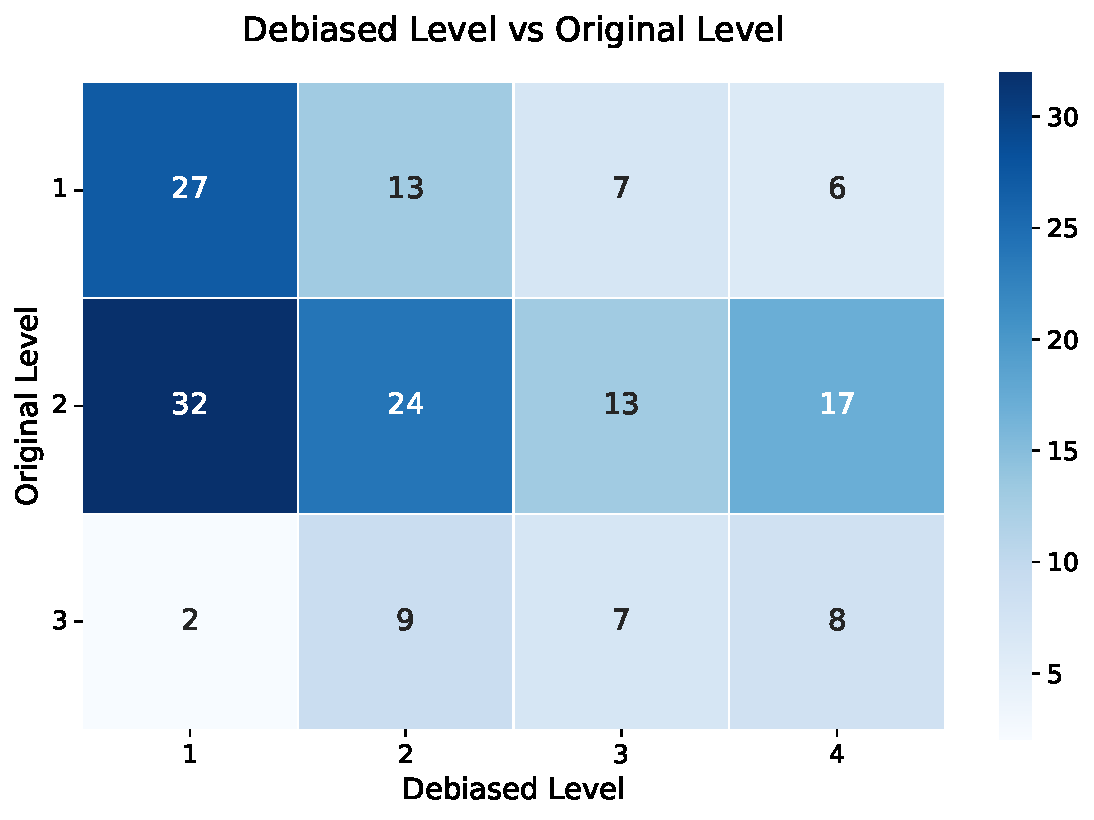
\includegraphics[width=0.5\linewidth]{figs/levels_heatmap.pdf}
    \caption{The distribution between original level and reassigned level.}
    \label{fig:debias}
\end{figure}

In addition, we observe that recent progress in enhancing agentic capabilities of open-source models through reinforcement learning has been rapid, achieving high scores on the \gaia{} benchmark and substantially improving efficiency. This provides a highly promising direction for our future work.
\begin{table}[!h]
\centering%\small
\setstretch{1.1}
\caption{Performance comparison of various base models on \gaia{} benchmark. All results are obtained using information retrieved from Google Search.}
\label{tab:crawler}
\vspace{-9pt}
\begin{tabular}{l|cccc}
\toprule
Model & Average & Level 1 & Level 2 & Level 3  \\
\midrule
WebShaper-32B & 53.3 & 69.2 & 50.0 & 16.6 \\
WebShaper-72B & 60.1 & 69.2 & 63.4 & 16.6 \\
\midrule
GPT-4.1 & 55.8 & 66.0 & 58.1 & 26.9 \\
o4-mini & 66.1 & 79.2 & 68.6 & 30.8 \\
Claude-3.7-sonnet & 68.3 & 83.1 & 70.6 & 30.8 \\
Claude-4-sonnet & 75.2 & 86.6 & 77.9 & 42.3 \\
\bottomrule
\end{tabular}
\end{table}

\begin{table}[!h]
\centering
\setstretch{1.2}
\caption{Performance of various search engine settings on \gaia{}. Note that `Multi-Source' refers to combine the above search engines.}
\vspace{-9pt}
\label{tab:search}
\begin{tabular}{l|cccc}
\toprule
Search Method & Average & Level 1 & Level 2 & Level 3  \\
\midrule
Google        & 75.2 & 86.6 & 77.9 & 42.3 \\
Bing          & 58.8 & 62.3 & 64.0 & 34.6 \\
DuckDuckGo    & 70.9 & 81.1 & 73.3 & 42.3 \\
Multi-Source  & 68.5 & 75.5 & 73.3 & 38.5 \\
\bottomrule
\end{tabular}
\end{table}



\noindent \textbf{Search Engine}
Web search is significant for LLM-agents to obtain external information beyond their knowledge boundaries. However, we found that different search engines and search engine service APIs have substantial impacts on task performance. We employed Google, Bing, DuckDuckGo, and their aggregated results (Multi-Source) respectively. As shown in Table~\ref{tab:search}, Agent with Google achieved the highest score of 75.2. Beyond differences in search result entries, a possible explanation is that Google (supported by SerpAPI) provides more fine-grained filtering condition settings, including date, location,  specific categories etc. For the GAIA benchmark, such fine-grained conditional filtering is essential.


\subsubsection{Level Debias}
The difficulty level assignments for tasks in the GAIA dataset rely as a proxy on the number of steps and tools used by our annotators when crafting the questions. However, there exists a gap between human behavior and machine behavior, where tasks that are simple for humans—such as visual recognition and browser operations—are indeed more challenging for machines. Therefore, we have reclassified them into four levels based on problem-solving success rates under our agent system, as shown in Fig~\ref{fig:debias}.

